%\documentclass[12pt,mathserif,dvipdfmx,aspectratio=32]{beamer}
\documentclass[12pt,dvipdfmx,mathserif,uplatex,aspectratio=32]{beamer}
%\usepackage[dvipdfmx]{graphicx}
\usepackage{atbegshi}
\AtBeginShipoutFirst{\special{pdf:tounicode EUC-UCS2}}
%\AtBeginShipoutFirst{\special{pdf:tounicode 90ms-RKSJ-UCS2}}
\usepackage{minijs}
%\usepackage{oft}
\renewcommand{\kanjifamilydefault}{\gtdefault}
\usetheme{default}
%\usetheme{Antibes}
%\usecolortheme{albatross}
\setbeamertemplate{navigation symbols}{}
\setbeamercolor{frametitle}{fg=blue}
\setbeamercolor{title}{fg=black}
\setbeamercolor{table}{fg=black}
\setbeamersize{text margin right=0.5cm}
\setbeamersize{text margin left=0.5cm}
%\setbeamerfont{euler}
%\usepackage{eulervm}
\usepackage{euler}
\usepackage{multicol}
\usepackage{subfigure}

%%
%% プリアンブルに記述
%% Figure 環境中で Table 環境の見出しを表示・カウンタの操作に必要
%%
\makeatletter
\newcommand{\figcaption}[1]{\def\@captype{figure}\caption{#1}}
\newcommand{\tblcaption}[1]{\def\@captype{table}\caption{#1}}
\makeatother


%\title{決定木を用いた \\ Run-Based Trieの探索法}
\title{Run-Based Trie を用いた \\ パケットフィルタリングアルゴリズム}
\subtitle{\empty}
%\subtitle{すべてわかるSDN大全p90$\sim$p92}
%\vspace{30mm}
\author[氏名略称]{原田崇司}
\institute[所属略称]{{\normalsize 神奈川大学大学院 理学研究科 情報科学専攻 田中研究室}}
%\date{2014年9月26日}
\date{\empty}
%
% contents
%
\begin{document}

%% \begin{frame}
%%  \titlepage
%% \end{frame}

%% %
%% \section*{内容}
%%  \begin{frame}{目次}
%%   \tableofcontents
%%  \end{frame}
%% %

%% \section{Packet Filtering と Run-Based Trie}
%% %1枚目

%% \begin{frame}{パケットフィルタリング}
%% %話がフィルタリングについてであることを言う.
%% \begin{figure}
%%  \centering{
%%   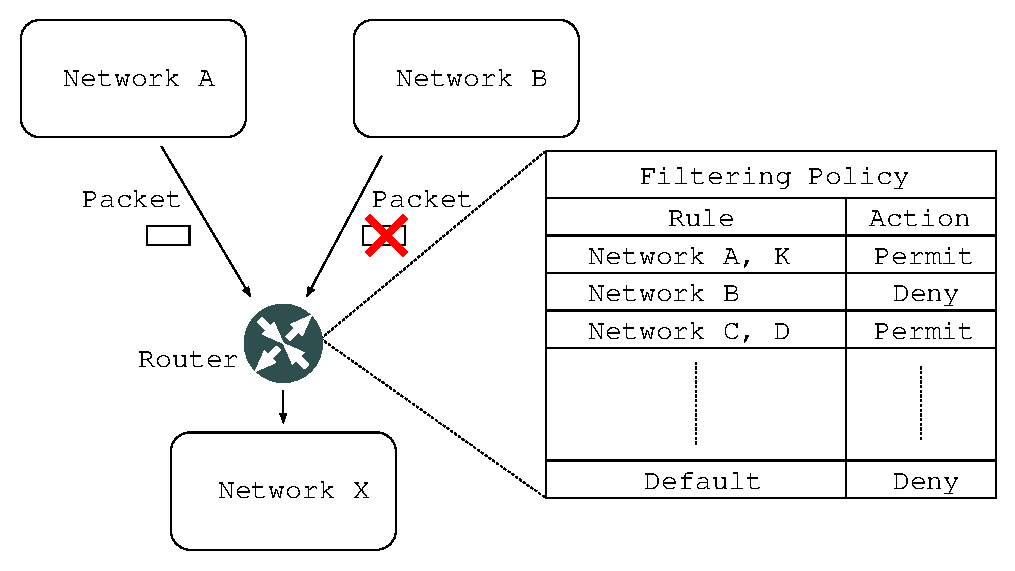
\includegraphics[scale=0.65]{filter-example.eps}
%%  }
%% \par
%% \vspace{5mm}
%% 入ってくるパケットをポリシーに従ってルータで分類
%% \end{figure}
%% \end{frame}


%% %2枚目
%% \begin{frame}{パケットフィルタリングの方法}
%% \vspace{1mm}
%% \hspace{1mm} {\large \textbf{線型探索}} \hspace{48mm} {\large \textbf{その他}}
%% \vspace{2mm}
%% \begin{figure}
%%  \centering{
%%   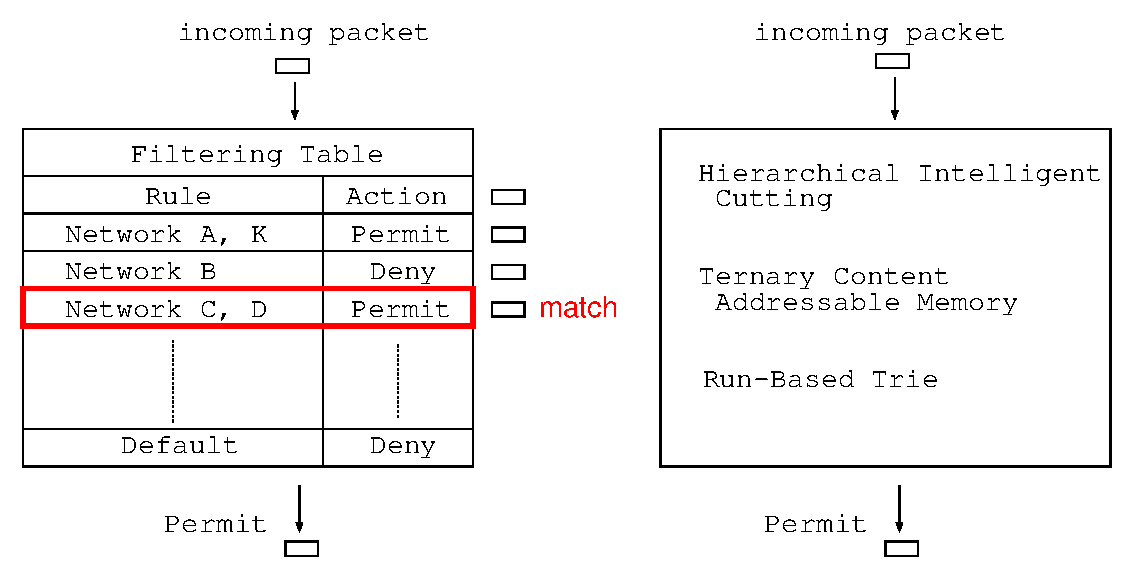
\includegraphics[scale=0.65]{filtering.eps}
%%  }
%% \end{figure}
%% \end{frame}


%% %3枚目
%% \begin{frame}{Run-Based Trie(三河,田中,2015)}

%% \vspace{1mm}
%% {\large \color{black}連の開始位置$i$ビット目ごとにトライ$T_{i}$を構成
%% }
%% \vspace{2mm}

%% \begin{figure}[h]
%% \begin{flushleft}
%%  \def\@captype{table}
%%  \begin{minipage}[t]{.38\textwidth}
%%   \begin{center}
%%   \begin{tabular}{ccc}
%%         & &    \\ \hline
%%  $Filter$ & & $F$ \\ \hline
%%  $R_{1}$ & & $0$ $*$ $1$ \\ 
%%  $R_{2}$ & & $*$ $0$ $0$ \\ 
%%  $R_{3}$ & & $1$ $1$ $0$ \\ 
%%  $R_{4}$ & & $1$ $1$ $*$ \\ 
%%  $R_{5}$ & & $0$ $*$ $*$ \\ 
%%  $R_{6}$ & & $*$ $1$ $*$ \\ \hline
%%   \end{tabular}
%%   \end{center}
%%  %\tblcaption{左側の表の見出し}
%%  %\label{左側の表へのラベル}
%%  \end{minipage}
%%  \hfill
%%  %
%%  \begin{minipage}[c]{.60\textwidth}
%%  %\caption{Run-Based Trie}
%%  \scalebox{0.7}{\input{rbtrie.tps}}
%% %\label{図へのラベル}
%%  \end{minipage}
%% \end{flushleft}
%% \end{figure}


%% \end{frame}



%% %4枚目
%% \begin{frame}{Simple Search でパケット $111$ を分類}
%% \vspace{3mm}

%% \begin{figure}[h]
%% \begin{center}
%%  \def\@captype{table}
%%  \begin{minipage}[t]{.48\textwidth}
%%   \begin{center}
%%   \begin{tabular}{ccc}
%%         & &    \\ \hline
%%  $Filter $& & $F$ \\ \hline
%%  $R_{1}$ & & $0$ $*$ $1$ \\ 
%%  $R_{2}$ & & $*$ $0$ $0$ \\ 
%%  $R_{3}$ & & $1$ $1$ $0$ \\ 
%%  {\color{red} $R_{4}$} & & {\color{red} $1$ $1$} $*$ \\ 
%%  $R_{5}$ & & $0$ $*$ $*$ \\ 
%%  $R_{6}$ & & $*$ $1$ $*$ \\ \hline
%%   \end{tabular}
%%   \end{center}
%%  %\tblcaption{左側の表の見出し}
%%  %\label{左側の表へのラベル}
%%  \end{minipage}
%%  \hfill
%%  %
%%  \begin{minipage}[c]{.40\textwidth}
%%  %\caption{Run-Based Trie}
%%  \scalebox{0.7}{\input{nsimple1.tps}}
%% %\label{図へのラベル}
%%  \end{minipage}
%% \end{center}
%% \end{figure}

%% \vspace{10mm}
%% \centering{
%%   \begin{tabular}{|c|c|c|c|c|c|c|} \hline
%%  最優先ルール & $R_{1}$ &  $R_{2}$ &  $R_{3}$ &  $R_{4}$ &  $R_{5}$ &  $R_{6}$ \\ \hline
%%  $7$ $\rightarrow$ {\color{red} $4$} & $0$ & $0$ & $0$ & $0$ $\rightarrow$ {\color{red}$1$} & $0$ & $0$ \\ \hline 
%%   \end{tabular}
%% %合致しているルール $\{ R_{5} \}$,現在の最優先ルール $R_{5}$
%% }
%% \end{frame}

%% %5枚目
%% \begin{frame}{Simple Search でパケット $111$ を分類}

%% \begin{figure}[h]
%% \begin{center}
%%  \def\@captype{table}
%%  \begin{minipage}[t]{.48\textwidth}
%%   \begin{center}
%%   \begin{tabular}{ccc}
%%         & &    \\ \hline
%%  $Filter $& & $F$ \\ \hline
%%  $R_{1}$ & & $0$ $*$ $1$ \\ 
%%  $R_{2}$ & & $*$ $0$ $0$ \\ 
%%  $R_{3}$ & & $1$ $1$ $0$ \\ 
%%  $R_{4}$ & & $1$ $1$ $*$ \\ 
%%  $R_{5}$ & & $0$ $*$ $*$ \\ 
%%  {\color{red} $R_{6}$} & & $*$ {\color{red} $1$} $*$ \\ \hline
%%   \end{tabular}
%%   \end{center}
%%  %\tblcaption{左側の表の見出し}
%%  %\label{左側の表へのラベル}
%%  \end{minipage}
%%  \hfill
%%  %
%%  \begin{minipage}[c]{.40\textwidth}
%%  %\caption{Run-Based Trie}
%%  \scalebox{0.7}{\input{simple2.tps}}
%% %\label{図へのラベル}
%%  \end{minipage}
%% \end{center}
%% \end{figure}

%% \vspace{10mm}
%% \centering{
%%   \begin{tabular}{|c|c|c|c|c|c|c|} \hline
%%  最優先ルール & $R_{1}$ &  $R_{2}$ &  $R_{3}$ &  $R_{4}$ &  $R_{5}$ &  $R_{6}$ \\ \hline
%%   $4$ & $0$ & $0$ & $0$ & $1$ & $0$ & $0$ $\rightarrow$ {\color{red}$1$} \\ \hline 
%%   \end{tabular}
%% %合致しているルール $\{ R_{5} \}$,現在の最優先ルール $R_{5}$
%% }

%% \end{frame}


%% %6枚目
%% \begin{frame}{Simple Search でパケット $111$ を分類}

%% \begin{figure}[h]
%% \begin{center}
%%  \def\@captype{table}
%%  \begin{minipage}[t]{.58\textwidth}
%%   \begin{center}
%%   \begin{tabular}{ccc}
%%         & &    \\ \hline
%%  $Filter $& & $F$ \\ \hline
%%  $R_{1}$ & & $0$ $*$ ${\color{red}{1}}$ \\ 
%%  $R_{2}$ & & $*$ $0$ $0$ \\ 
%%  $R_{3}$ & & $1$ $1$ $0$ \\ 
%%  $R_{4}$ & & $1$ $1$ $*$ \\ 
%%  $R_{5}$ & & $0$ $*$ $*$ \\ 
%%  $R_{6}$ & & $*$ $1$ $*$ \\ \hline
%%   \end{tabular}
%%   \end{center}
%%  %\tblcaption{左側の表の見出し}
%%  %\label{左側の表へのラベル}
%%  \end{minipage}
%%  \hfill
%%  %
%%  \begin{minipage}[c]{.40\textwidth}
%%  %\caption{Run-Based Trie}
%%  \scalebox{0.7}{\input{nsimple3.tps}}
%% %\label{図へのラベル}
%%  \end{minipage}
%% \end{center}
%% \end{figure}

%% %\vspace{5mm}
%% \centering{
%%   \begin{tabular}{|c|c|c|c|c|c|c|} \hline
%%  最優先ルール & $R_{1}$ &  $R_{2}$ &  $R_{3}$ &  $R_{4}$ &  $R_{5}$ &  $R_{6}$ \\ \hline
%%  $4$ & $0$ {\color{red}$\nrightarrow$} $2$ & $0$ & $1$ & $1$ & $0$ & $1$ \\ \hline 
%%   \end{tabular}
%% }

%% \vspace{5mm}

%% 探索終了.パケット$111$に合致する最優先ルールは $R_{4}$

%% \end{frame}



%% \section{Pointed Run-Based Trie}
%% %7枚目
%% \begin{frame}{Pointed Run-Based Trie}

%% \centering{

%%  \scalebox{0.6}{\input{srbtrie.tps}}

%% }

%% \vspace{5mm}

%% パケット$111$を Simple Search で探索すると,ノードと6回比較 \\

%% \vspace{3mm}

%% しかし,$T_{1}$ を $111$ と辿った時点で,$T_{2}$, $T_{3}$ をどう辿るかは分かる. \\

%% \vspace{5mm}

%% $\rightarrow$ $T_{2}$と$T_{3}$でのそれぞれ 1回,2回の比較を無くしたい

%% \end{frame}


%% %8枚目
%% \begin{frame}{Pointed Run-Based Trie}

%% 下位のトライ$T_{j}$の持つ連を上位のトライの$T_{i}$へ付与

%% \vspace{5mm}

%% {\centering

%%  \scalebox{0.6}{\input{prbtrie0.tps}}

%% }

%% \vspace{5mm}

%% {\centering
%% $T_{1}$を$11$と辿るパケットは,$T_{2}$を$1$と辿り$\underline{R_{6}^{1}}$を得る.\\
%% \vspace{3mm}
%% $\rightarrow$ $T_{1}$の$11$のノードへ${\color{red} \underline{R_{6}^{1}}}$を付与する \\
%% \vspace{3mm}
%% $\rightarrow$ $T_{2}$のRootから$1$の部分を辿らなくて良い.

%% }
%% \end{frame}

%% %9枚目
%% \begin{frame}{Pointed Run-Based Trie}

%% 上位のトライ$T_{i}$から下位のトライへポインタを張る($T_{1}$の$0$は省略)

%% \vspace{5mm}

%% {\centering

%%  \scalebox{0.6}{\input{prbtrie1.tps}}

%% }

%% \vspace{5mm}

%% {\centering
%% Simple Search は,$T_{i}$を辿れなくなったら,$T_{i+1}$の根を始点に辿る.\\
%% \vspace{3mm}
%% Ponited Run-Based Trieは,$T_{1}$の根から始め,\\ \vspace{3mm} 辿れなくなったら,探索終了.

%% }
%% \end{frame}

%% %10枚目
%% \begin{frame}{Pointed Run-Based Trie}


%% \vspace{5mm}

%% {\centering

%%  \scalebox{0.6}{\input{prbtrie2.tps}}

%% }

%% \vspace{10mm}

%% {\centering
%% Pointed Run-Based Trie を用いた探索.最優先ルールは,$R_{4}$

%% }
%% \end{frame}

\section{決定木を用いた Run-Based Trie の探索法}
%11枚目
\begin{frame}{集合族(Simple Searchでの$T_{i}$の辿り方の場合分け)}
\vspace{-3mm}
\centering{
 \scalebox{0.6}{\input{rbtrie.tps}}
}
\vspace{-2mm}
 \begin{align*}
  S_{1} &= \{\{ R_{1}^{1}, \ \underline{ R_{5}^{1}} \}, \ \{ \underline{ R_{4}^{1}} \}, \ \{\underline{ R_{3}^{1}}, \ \underline{ R_{4}^{1}} \}, \ \phi \}  \\
  S_{2} &= \{ \{ \underline{ R_{2}^{1}} \}, \ \{ \underline{ R_{6}^{1}} \}, \ \phi \}  \\
  S_{3} &= \{ \{ \underline{ R_{1}^{2}} \}, \ \phi \} 
 \end{align*}
集合族の直積$|S_{1}| \times |S_{2}| \times |S_{3}|$を取り,対応するルールを付与 \\ 
\vspace{1mm}
%$\rightarrow$ 
連の合致の組み合わせを全て列挙
\end{frame}

%% %12枚目
%% \begin{frame}{決定木}
%% %\vspace{10mm}
%%  \centering{
%%   \scalebox{0.8}{\input{dtree.tps}}
%%  }
%%  \par

%% {\color{red}{Run-Based Trieに従って決定木を辿るだけで,パケットを分類可能}} \\
%% \vspace{3mm}
%% (連の照合,合致ルール間の優先度の比較をしなくて良い)

%% \end{frame}


%13枚目
\begin{frame}{決定木によりパケット$111$を探索}
% 各集合族 $S_{i}^{j}$ を,対応するビット列でラベル付けする.
%\vspace{10mm}
 \centering{
  \scalebox{0.8}{\input{dtreenum.tps}}
 }
 \par

Run-Based Trie を用いて決定木を辿る.最優先ルールは $R_{4}$\\
\vspace{3mm}

しかし,不要なパス,ノードが大量発生 $\rightarrow$ {\color{red}決定木の枝刈り}が必要
\end{frame}


%14枚目
\begin{frame}{各集合のビット列のラベルを参照}

 {\centering

  \scalebox{0.8}{\input{delete1.tps}}

 }

\vspace{5mm}
{\centering
$11$のノードは,次のトライを$1$と辿ることを意味する.
}

{\centering

\begin{itemize}
 \item 下位のトライを$00$と辿ることはない.
 \item 下位の集合族に$1$があるので,下位のトライを$1$と辿り,\\ \vspace{1mm} 連を獲得しない($\phi$)ということはない.
\end{itemize}

}
\end{frame}

%15枚目
\begin{frame}{集合族$S_{k}$内の集合$S_{k}^{l}$と$S_{k}^{m}$のラベルを比較}

 {\centering

  \scalebox{0.8}{\input{delete2.tps}}

 }

\vspace{3mm}

{\centering
$11$の高さに$110$がある $\rightarrow$ $11$の子孫に,$110$に対応するノードは不要 \\
\vspace{3mm}
}


\end{frame}


%% \section{実験結果}

%% %枚目
%% \begin{frame}{実験結果}

%%  %% \centering{
%%  %%  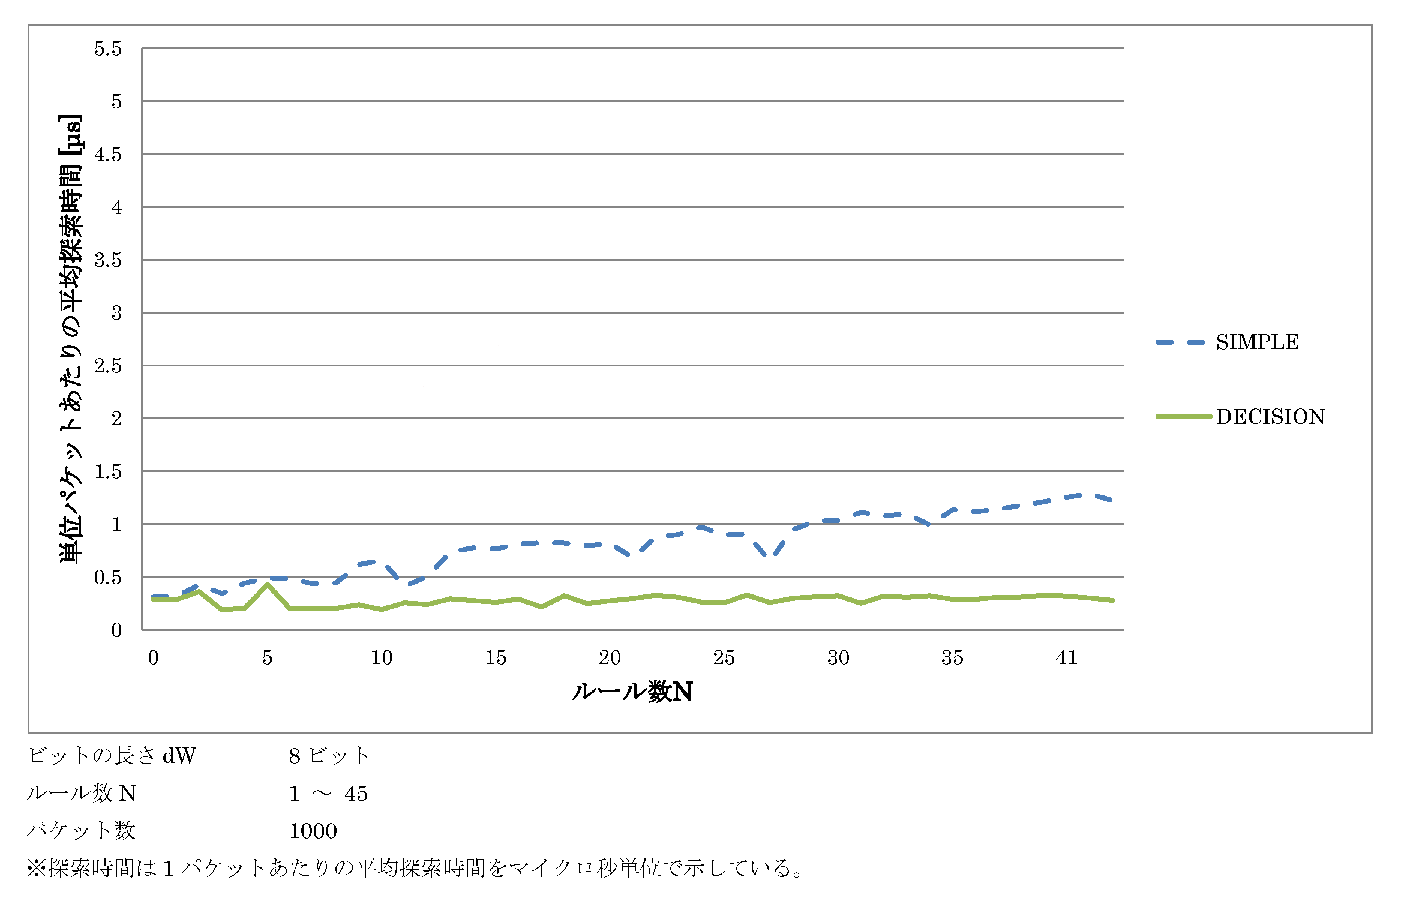
\includegraphics[scale=0.5]{result2.eps}
%%  %% }
%% \end{frame}


%% \section{まとめと今後の課題}
%% %枚目
%% \begin{frame}{まとめ}

%%  \begin{itemize}
%%   \item Run-Based Trie のノードにポインタを適当に張ることにより,\\ \vspace{3mm} 探索時間計算量が $O(dW^{2} + NdW)$ から $O(NdW)$ へ減少 \vspace{10mm}
%%   \item 決定木を用いて Run-Based Trie を探索することにより,\\ \vspace{3mm} フィルタリングルールの数$N$に依存せず探索可能
%%  \end{itemize}

%% %%  {\large 今後の課題}

%% %%  \vspace{3mm}
%% %%  \begin{itemize}
%% %%   \item Simple Searchの全ての辿り方を組み合わせるので,\\ 
%% %% 決定木の空間計算量が膨大 $\rightarrow$ 枝刈りアルゴリズムが必要
%% %%   \vspace{3mm}
%% %%   \item 決定木の空間計算量の算出
%% %%   \vspace{3mm}
%% %%   \item プログラムを作成して,$16$ビット以上での実装実験
%% %%  \end{itemize}

%% \end{frame}

%% \begin{frame}{今後の課題}

%% \end{frame}



%%%%%%%%%%%%%%%%%%%%%%%%%%%%%%%%%%%%%%%%%%%%%%%%%%%%%%%%%%%%%%%%


%
% \section*{references}
% \begin{frame}[allowframebreaks]{References}
%  \scriptsize
%  \bibliographystyle{jplain}
%  \bibliography{ebibtex}
% \end{frame}
 %
% \slide{ご清聴ありがとうございました.}
%
\end{document}
